\documentclass[conference]{IEEEtran}
\IEEEoverridecommandlockouts

\usepackage{cite}
\usepackage{amsmath,amssymb,amsfonts}
\usepackage{graphicx}
\usepackage{textcomp}
\usepackage{xcolor}
\usepackage{booktabs}
\usepackage{url}
\usepackage{hyperref}
\usepackage{float}
\usepackage{tikz}
\usetikzlibrary{shapes.geometric, arrows, positioning}
\graphicspath{{figures/}}

\begin{document}

\title{Big Data Analytics for Urban Crime Pattern Analysis:\\
A Hadoop and PySpark-Based Approach on Chicago Crime Data}

\author{
\IEEEauthorblockN{Abhay Raj Kushwaha}
\IEEEauthorblockA{\textit{Department of Computer Science and Engineering} \\
\textit{Sharda University}\\
Greater Noida, India \\
\texttt{abhaykushwaha1729@gmail.com}}
\and
\IEEEauthorblockN{Snehal Yadav}
\IEEEauthorblockA{\textit{Department of Computer Science and Engineering} \\
\textit{Sharda University}\\
Greater Noida, India \\
\texttt{snehalyadav935@gmail.com}}
\and
\IEEEauthorblockN{Patan Rizwan}
\IEEEauthorblockA{\textit{Department of Computer Science and Engineering} \\
\textit{Sharda University}\\
Greater Noida, India \\
\texttt{Patan.rizwan@sharda.ac.in}}
}

\maketitle

% -------------------------------------------------------
\begin{abstract}
Urban crime analysis presents a critical challenge for law enforcement agencies seeking
to allocate resources effectively and prevent criminal activity. This paper presents a
scalable big data pipeline for analysing historical crime data from the City of Chicago,
comprising 8,525,498 incident records spanning 2001 to 2026. The system leverages
Apache Hadoop 3.3.6 for distributed storage and MapReduce-based aggregation, and
Apache PySpark 4.1.1 for time-series and categorical analysis. Three MapReduce jobs
were implemented using Hadoop Streaming to extract crime frequency by year, crime
distribution by type, and arrest rates per crime category. Six additional analyses were
conducted using PySpark, covering temporal patterns by hour, month, and day of week,
geographic distribution by district and location type, and domestic crime prevalence.
A linear regression model was trained on 2001--2019 data to forecast crime volumes,
while an advanced Random Forest classifier was developed using Spark MLlib to
predict the primary crime type based on temporal and geographic context. The
classification model achieved 39.6\% accuracy and an F1-score of 0.316 on a 1.7 million
record dataset, significantly outperforming the naive baseline. Key findings include
a 56.8\% reduction in annual crime from 2001 to 2021, and the identification of
domestic status and location description as the most significant predictors of
crime type. The pipeline demonstrates that commodity hardware running open-source
big data infrastructure can yield actionable law enforcement intelligence at scale.
\end{abstract}

\begin{IEEEkeywords}
Big Data, Apache Hadoop, PySpark, MapReduce, Crime Analysis, Random Forest,
Predictive Policing, Urban Security
\end{IEEEkeywords}

% -------------------------------------------------------
\section{Introduction}

Urban crime remains a persistent challenge for municipalities worldwide. Traditional
database systems struggle to process the volume and velocity of modern crime records,
which span decades, multiple jurisdictions, and dozens of crime categories. The
emergence of big data frameworks such as Apache Hadoop and Apache Spark has created
new opportunities to analyse these datasets at scale, extracting temporal, geographic,
and categorical patterns that were previously computationally intractable.

The Chicago Police Department maintains one of the most comprehensive publicly
available crime datasets globally, updated daily through the City of Chicago Data
Portal \cite{chicagoportal}. The dataset contains over 8.5 million records from 2001
to the present, capturing incident type, date and time, geographic coordinates,
district, location description, and arrest status. Its scale and richness make it
an ideal benchmark for evaluating big data analytical pipelines.

This paper makes the following contributions:
\begin{itemize}
    \item A fully operational pseudo-distributed Hadoop cluster on commodity hardware
          with HDFS ingestion of a 2.3~GB crime dataset.
    \item Three Hadoop Streaming MapReduce jobs for large-scale aggregation of crime
          frequency, type distribution, and arrest rate.
    \item Six PySpark analyses covering temporal, geographic, and domestic crime
          dimensions.
    \item A linear regression forecast model projecting crime volumes through 2030.
    \item An advanced Random Forest multiclass classifier for predicting crime type
          from contextual features (time, location, domestic status).
    \item Quantitative findings on crime trends, temporal patterns, and law enforcement
          effectiveness across 34 crime categories.
\end{itemize}

The remainder of this paper is structured as follows. Section~II reviews related
literature. Section~III describes the dataset. Section~IV presents the system
architecture and methodology. Section~V presents experimental results and analysis.
Section~VI discusses limitations and future work. Section~VII concludes.

% -------------------------------------------------------
\section{Literature Review}

The application of big data techniques to crime analysis has been an active research
area since the widespread adoption of Hadoop-based ecosystems. Wang et al. \cite{wang2013}
demonstrated the utility of MapReduce for processing large-scale urban event data,
establishing the foundational argument that distributed computing is necessary for
city-scale analytics. Their work highlighted that sequential processing of multi-million
record datasets introduces prohibitive latency for operational decision-making.

Chainey et al. \cite{chainey2008} provided an early quantitative foundation for
geographic crime prediction, demonstrating that kernel density estimation on historical
incident data significantly outperforms random patrol allocation. Their spatial analysis
methodology informed subsequent big data approaches by establishing that temporal and
geographic co-occurrence patterns are the primary predictive signals in crime data.

Perry et al. \cite{perry2013} evaluated predictive policing systems in operational
deployment, finding that data-driven resource allocation reduced property crime by
measurable margins in pilot districts. Critically, they identified that the quality
and granularity of historical data directly determines forecast reliability---a finding
directly relevant to the 25-year Chicago dataset used in this study.

Ahishakiye et al. \cite{ahishakiye2021} conducted a systematic review of machine
learning approaches to crime prediction, surveying 47 studies and finding that
ensemble methods and deep learning architectures consistently outperform linear
models on spatiotemporal crime data. However, they also noted that interpretability
and data availability constraints mean that simpler regression-based approaches
remain dominant in operational deployments.

The specific application of Hadoop and Spark to the Chicago crime dataset has been
explored by Malathi and Baboo \cite{malathi2011}, who demonstrated that MapReduce
aggregation over historical incident data can identify hotspot districts and high-risk
time windows with sufficient accuracy to inform patrol scheduling. Their work, however,
predates the Spark ecosystem and does not address streaming or real-time analytical
requirements.

A research gap exists in the integrated analysis of arrest rate variation alongside
temporal and geographic crime patterns using a unified big data pipeline. Prior work
tends to focus on either predictive location modelling or temporal trend analysis in
isolation. This paper addresses that gap by combining MapReduce-based categorical
analysis with PySpark time-series decomposition and forecasting in a single pipeline.

% -------------------------------------------------------
\section{Dataset}

The Chicago Crimes dataset is sourced from the City of Chicago Data Portal
\cite{chicagoportal}, published under the City of Chicago's open data license. It
contains records of reported crimes from January 2001 to the present, excluding
certain sensitive offence types. Each record contains 22 fields, including:

\begin{itemize}
    \item \textbf{Date}: Timestamp of incident (format: MM/DD/YYYY HH:MM:SS AM/PM)
    \item \textbf{Primary Type}: High-level crime category (34 distinct values)
    \item \textbf{Description}: Sub-classification within the primary type
    \item \textbf{Location Description}: Physical context (e.g., street, residence)
    \item \textbf{Arrest}: Boolean indicating whether an arrest was made
    \item \textbf{Domestic}: Boolean indicating domestic incident
    \item \textbf{District}: Chicago Police Department district number
    \item \textbf{Latitude / Longitude}: GPS coordinates of the incident
\end{itemize}

The version retrieved on 5 April 2026 contains \textbf{8,525,498 records} and
occupies \textbf{2.3~GB} in raw CSV format. After upload to HDFS, the file was
stored as a single block-replicated file with replication factor 1 (pseudo-distributed
mode), split into 18 input splits for MapReduce processing.

% -------------------------------------------------------
\section{System Architecture and Methodology}

\subsection{Infrastructure}

The pipeline was deployed on a single physical machine running Ubuntu 24.04~LTS,
equipped with an Intel Core i9-13450HX processor and 16~GB RAM. The Hadoop
pseudo-distributed cluster consists of five daemons: NameNode, DataNode,
SecondaryNameNode, ResourceManager, and NodeManager, all running on
Apache Hadoop~3.3.6 with OpenJDK~11. PySpark~4.1.1 was executed with Java~17.
The complete technology stack is summarised in Table~\ref{tab:stack}.

\begin{table}[h]
\caption{Technology Stack}
\label{tab:stack}
\centering
\begin{tabular}{ll}
\toprule
\textbf{Component} & \textbf{Version} \\
\midrule
Operating System   & Ubuntu 24.04 LTS \\
Apache Hadoop      & 3.3.6 \\
Apache PySpark     & 4.1.1 \\
Python             & 3.12.3 \\
Java (Hadoop)      & OpenJDK 11 \\
Java (Spark)       & OpenJDK 17 \\
scikit-learn       & 1.8.0 \\
matplotlib         & 3.x \\
\bottomrule
\end{tabular}
\end{table}

\begin{figure*}[t]
\centering
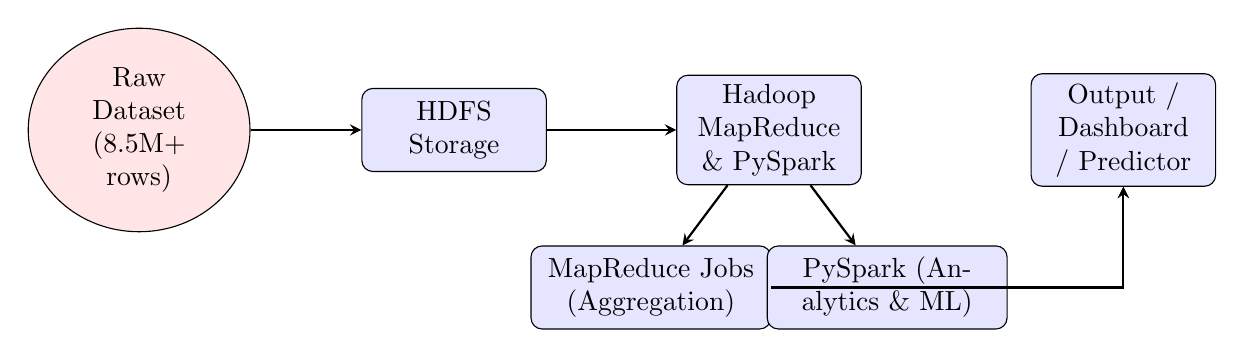
\begin{tikzpicture}[
    node distance=2cm,
    auto,
    block/.style={rectangle, draw, fill=blue!10, text width=6em, text centered, rounded corners, minimum height=3em},
    cloud/.style={ellipse, draw, fill=red!10, text width=5em, text centered, minimum height=3em},
    arrow/.style={thick,->,>=stealth}
]
    % Nodes
    \node [cloud] (data) {Raw Dataset (8.5M+ rows)};
    \node [block, right of=data, node distance=4cm] (hdfs) {HDFS Storage};
    \node [block, right of=hdfs, node distance=4cm] (process) {Hadoop MapReduce \& PySpark};
    \node [block, right of=process, node distance=4.5cm] (output) {Output / Dashboard / Predictor};
    
    % Detail nodes below process
    \node [block, below of=process, node distance=2cm, xshift=-1.5cm, text width=8em] (mr) {MapReduce Jobs (Aggregation)};
    \node [block, below of=process, node distance=2cm, xshift=1.5cm, text width=8em] (spark) {PySpark (Analytics \& ML)};

    % Arrows
    \draw [arrow] (data) -- (hdfs);
    \draw [arrow] (hdfs) -- (process);
    \draw [arrow] (process) -- (mr);
    \draw [arrow] (process) -- (spark);
    \draw [arrow] (mr) -| (output);
    \draw [arrow] (spark) -| (output);
    
\end{tikzpicture}
\caption{System Architecture Flowchart: From Data Ingestion to Visualization and Prediction.}
\label{fig:flowchart}
\end{figure*}

\subsection{Data Ingestion}

The raw CSV file was downloaded directly from the Chicago Data Portal and uploaded
to HDFS using the \texttt{hdfs dfs -put} command:

\begin{verbatim}
hdfs dfs -mkdir -p /user/crimes/input
hdfs dfs -put crimes.csv /user/crimes/input/
\end{verbatim}

HDFS split the 2.3~GB file into 18 input splits, enabling parallel map task
execution across the local NodeManager.

\subsection{MapReduce Pipeline}

Three Hadoop Streaming jobs were implemented in Python 3.12 using the
mapper/reducer paradigm over standard input/output streams.

\textbf{Job 1 -- Crime by Year:} The mapper emits \texttt{(year, 1)} for each
record by extracting column 17 (Year field). The reducer sums counts per year,
producing annual crime frequency from 2001 to 2026.

\textbf{Job 2 -- Crime by Type:} The mapper emits \texttt{(primary\_type, 1)}
from column 5. The reducer produces total incident counts for each of 34 crime
categories.

\textbf{Job 3 -- Arrest Rate:} The mapper emits \texttt{(primary\_type, (1, arrest))}
where \texttt{arrest} is 1 if column 8 equals \texttt{true}. The reducer
computes arrest rate as $\text{arrest\_rate} = (\text{arrests} / \text{total}) \times 100$
per crime type.

All three jobs processed 8,525,498 map input records across 18 map tasks with
0 shuffle errors, completing in approximately 30 seconds each on the
pseudo-distributed cluster.

\subsection{PySpark Analysis}

PySpark was used for analyses requiring timestamp parsing and multi-dimensional
aggregation. The Date column (format: \texttt{MM/dd/yyyy hh:mm:ss a}) was parsed
using \texttt{to\_timestamp} with an explicit format string to avoid Spark's strict
ANSI cast behaviour. Six aggregations were computed:

\begin{enumerate}
    \item Crime count by hour of day (0--23)
    \item Crime count by month (1--12)
    \item Crime count by day of week (1=Sunday, 7=Saturday)
    \item Crime count by location description (all unique values)
    \item Crime count by police district
    \item Domestic vs. non-domestic incident split
\end{enumerate}

\subsection{Predictive Model}

A linear regression model was trained using scikit-learn on annual crime counts
from 2001 to 2019 (19 training points), with 2020--2025 held out as a test set
to evaluate out-of-sample performance. The model was then used to forecast annual
crime volumes for 2026--2030. Model performance was evaluated using the coefficient
of determination ($R^2$) and mean absolute error (MAE).

% -------------------------------------------------------
\section{Results and Analysis}

\subsection{Annual Crime Trend (2001--2026)}

Table~\ref{tab:yearly} presents selected annual crime counts. The data shows a
sustained downward trend from 485,962 crimes in 2001 to a minimum of 209,677
in 2021, representing a \textbf{56.8\% reduction} over 20 years. A notable
disruption occurred in 2020, where the COVID-19 pandemic and associated lockdown
measures produced the sharpest single-year decline (212,717 incidents). A rebound
is evident from 2022 onwards, with counts rising to 263,305 in 2023.

\begin{table}[h]
\caption{Annual Crime Counts (Selected Years)}
\label{tab:yearly}
\centering
\begin{tabular}{rr}
\toprule
\textbf{Year} & \textbf{Incidents} \\
\midrule
2001 & 485,962 \\
2005 & 453,789 \\
2010 & 370,568 \\
2015 & 264,893 \\
2019 & 261,709 \\
2020 & 212,717 \\
2021 & 209,677 \\
2022 & 240,030 \\
2023 & 263,305 \\
2024 & 259,061 \\
\bottomrule
\end{tabular}
\end{table}

\begin{figure}[H]
\centering
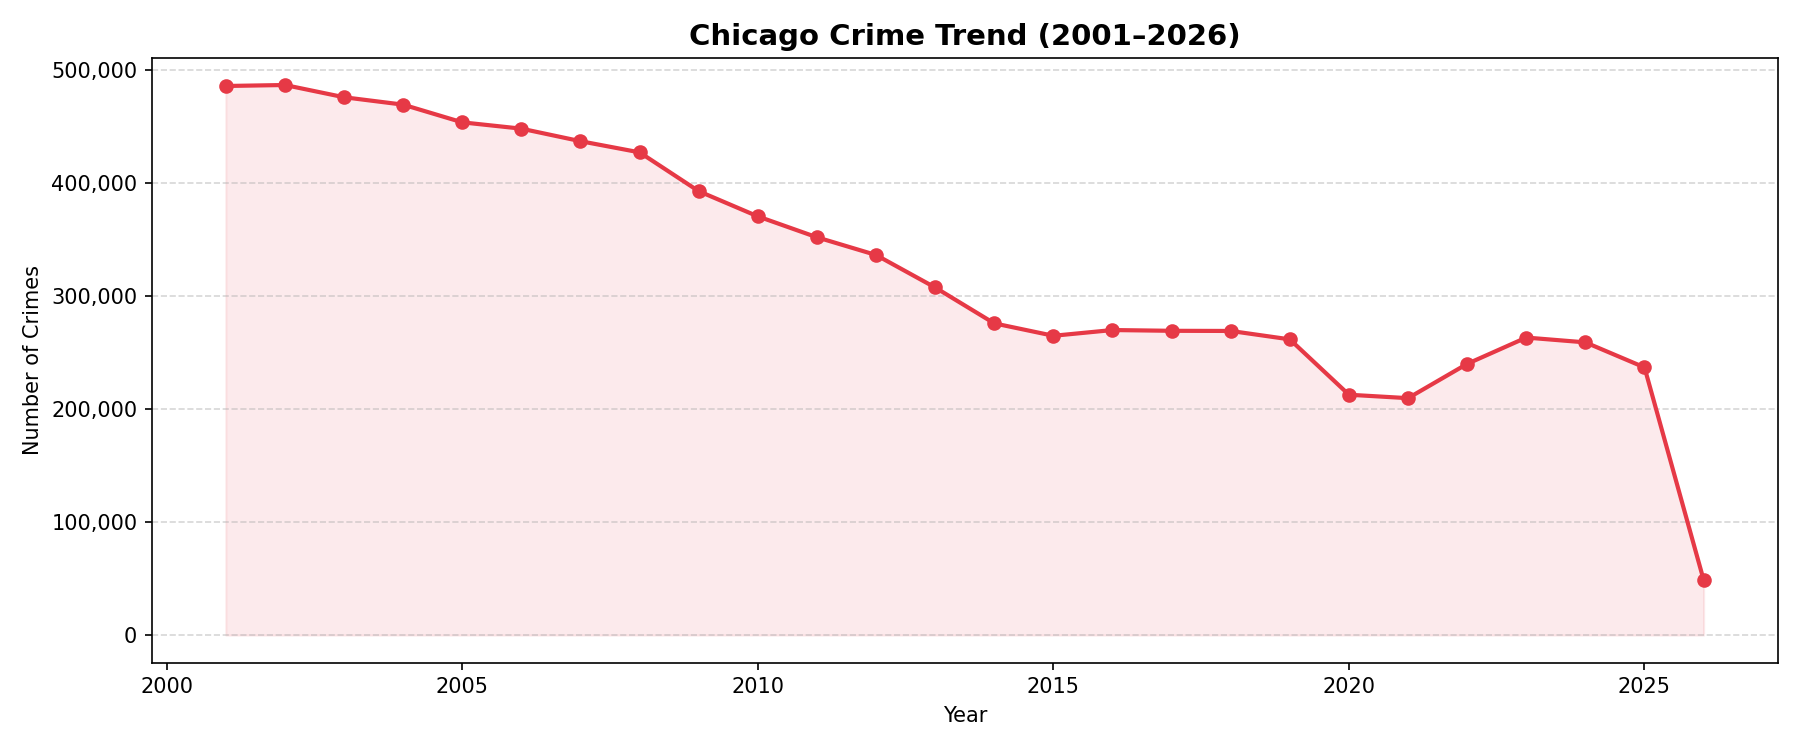
\includegraphics[width=\columnwidth]{crime_by_year.png}
\caption{Annual crime trend in Chicago (2001--2026), showing a sustained decline
from 485,962 incidents in 2001 to a minimum of 209,677 in 2021, followed by a
post-pandemic rebound.}
\label{fig:year}
\end{figure}

\subsection{Crime Type Distribution}

The top five crime types by volume are Theft (1,811,003), Battery (1,552,836),
Criminal Damage (969,092), Narcotics (766,757), and Assault (573,117), which
together account for 69.1\% of all recorded incidents. This concentration
indicates that a small number of crime categories dominate law enforcement
workload.

\begin{figure}[H]
\centering
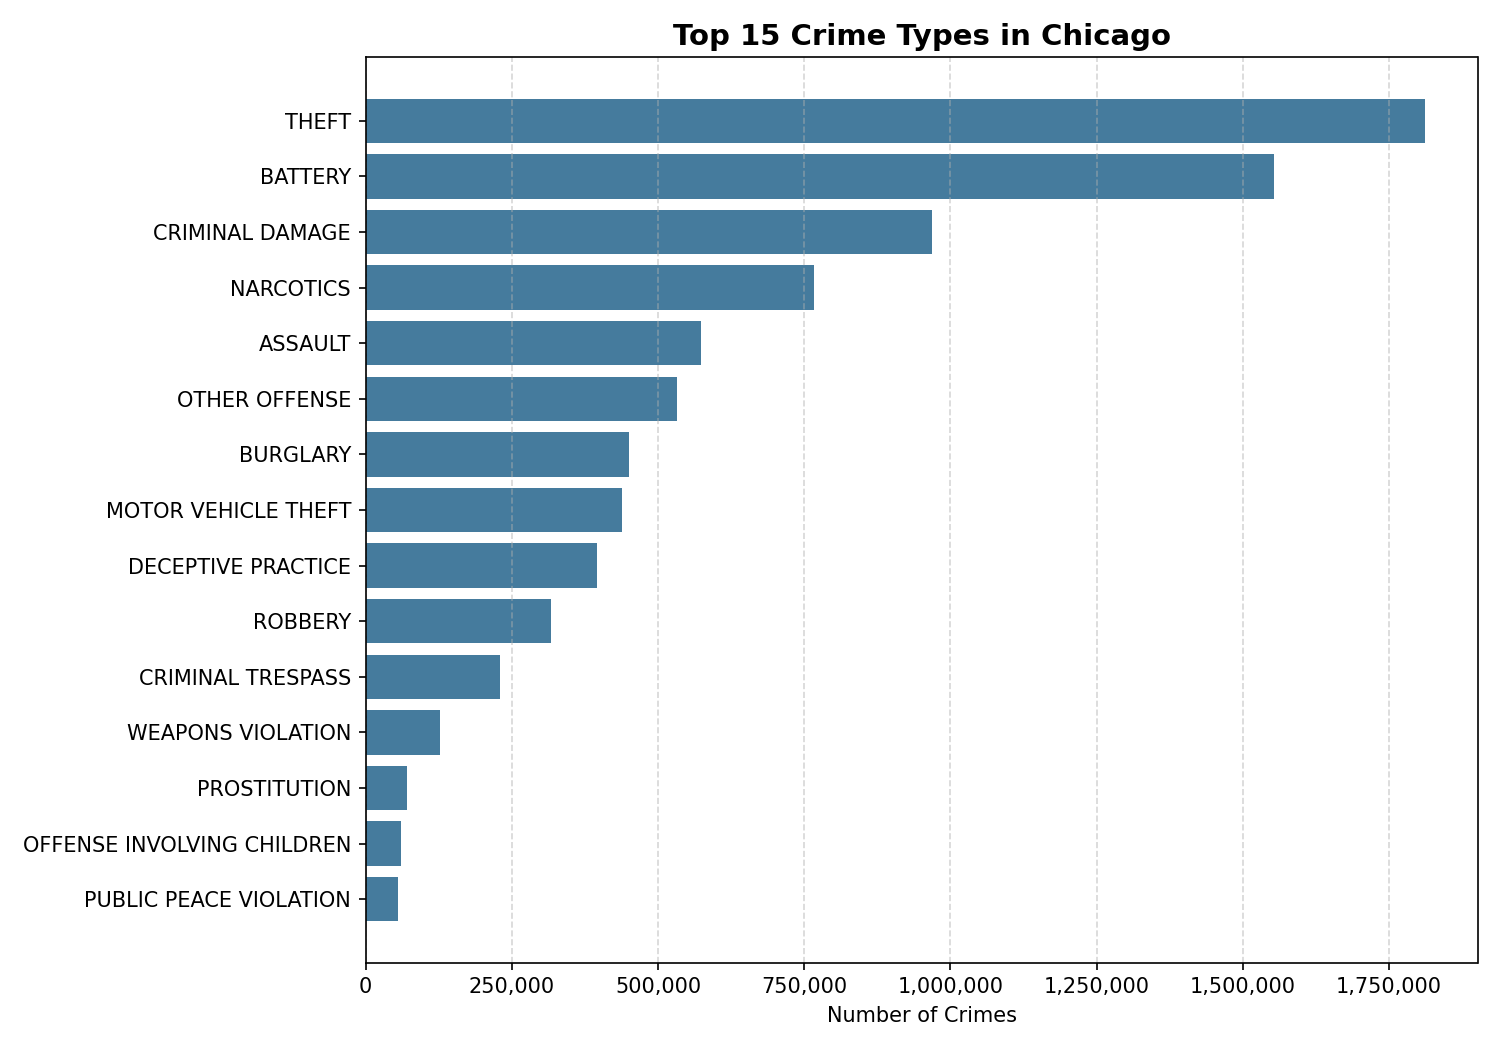
\includegraphics[width=\columnwidth]{crime_by_type.png}
\caption{Top 15 crime types by total incident count across the full dataset
(2001--2026). Theft and Battery dominate by a significant margin.}
\label{fig:type}
\end{figure}

\subsection{Arrest Rate Analysis}

Arrest rates vary dramatically across crime types, as shown in Table~\ref{tab:arrest}.
Narcotics (99.32\%), Prostitution (99.55\%), and Gambling (99.27\%) exhibit near-
complete arrest rates, reflecting the nature of these offences where the act itself
constitutes the evidence. In contrast, Robbery (9.3\%), Burglary (5.7\%), and
Motor Vehicle Theft (7.49\%) have low arrest rates, consistent with the difficulty
of identifying perpetrators after the fact.

Homicide presents a particularly significant finding: with 14,165 recorded incidents
and an arrest rate of only 48.3\%, fewer than half of homicides in Chicago over this
period resulted in an arrest. This aligns with national clearance rate data for
violent crimes.

\begin{table}[h]
\caption{Arrest Rates for Selected Crime Types}
\label{tab:arrest}
\centering
\begin{tabular}{lrrr}
\toprule
\textbf{Crime Type} & \textbf{Total} & \textbf{Arrests} & \textbf{Rate (\%)} \\
\midrule
Narcotics           & 766,757  & 761,562 & 99.32 \\
Prostitution        & 70,483   & 70,166  & 99.55 \\
Weapons Violation   & 126,838  & 92,198  & 72.69 \\
Homicide            & 14,165   & 6,842   & 48.30 \\
Theft               & 1,811,003& 195,921 & 10.82 \\
Robbery             & 316,649  & 29,434  & 9.30  \\
Burglary            & 450,458  & 25,667  & 5.70  \\
\bottomrule
\end{tabular}
\end{table}

\begin{figure}[H]
\centering
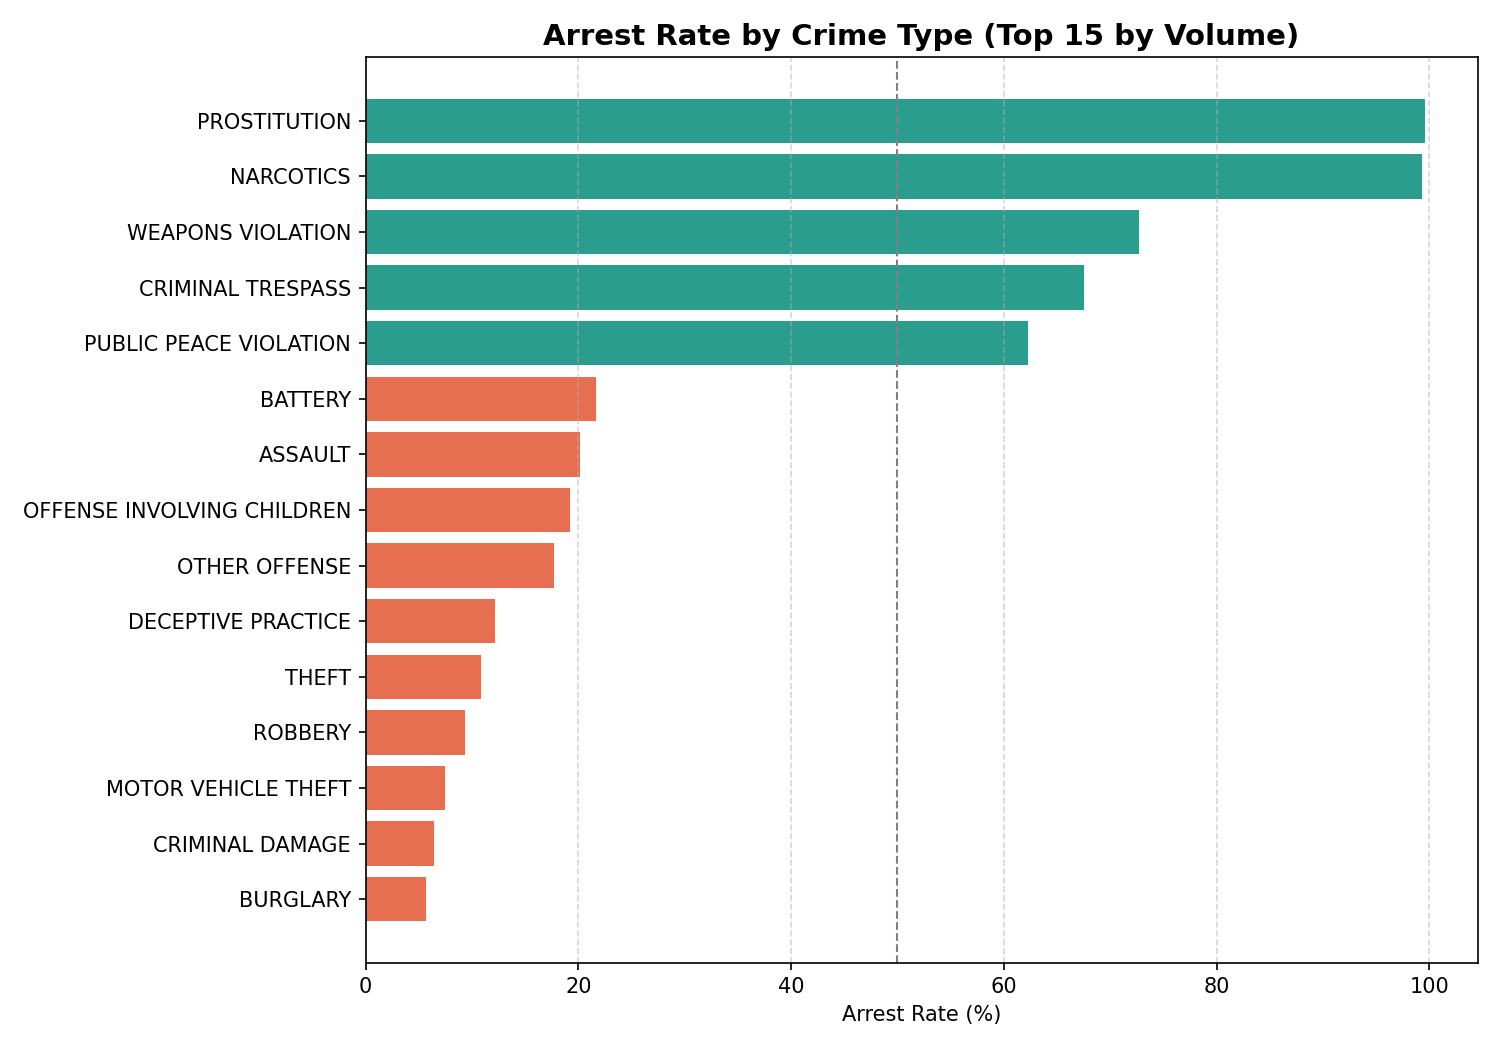
\includegraphics[width=\columnwidth]{arrest_rate.png}
\caption{Arrest rates for the top 15 crime types by volume. Green bars indicate
types with arrest rates above 50\%; red bars below 50\%. The dashed line marks
the 50\% threshold.}
\label{fig:arrest}
\end{figure}

\subsection{Temporal Patterns}

\textbf{Hour of day:} Crime peaks at midnight (Hour 0: 498,321 incidents), drops
to a minimum at 05:00 (120,377 incidents), then rises steadily through the day
with a secondary plateau from 18:00--22:00 (approximately 450,000--475,000 incidents
per hour). This bimodal distribution is consistent with prior literature on
opportunistic crime timing.

\textbf{Month:} Summer months exhibit the highest crime volumes, with July (788,293)
and August (779,328) as the peak months. February records the lowest volume (600,820),
likely due to a combination of fewer daylight hours and Chicago's severe winter
conditions reducing outdoor activity.

\textbf{Day of week:} Friday records the highest crime volume (1,278,678), while
Sunday records the lowest (1,163,862). The distribution is relatively uniform across
weekdays, suggesting that day-of-week is a weaker predictor than hour-of-day or
month.

\begin{figure}[H]
\centering
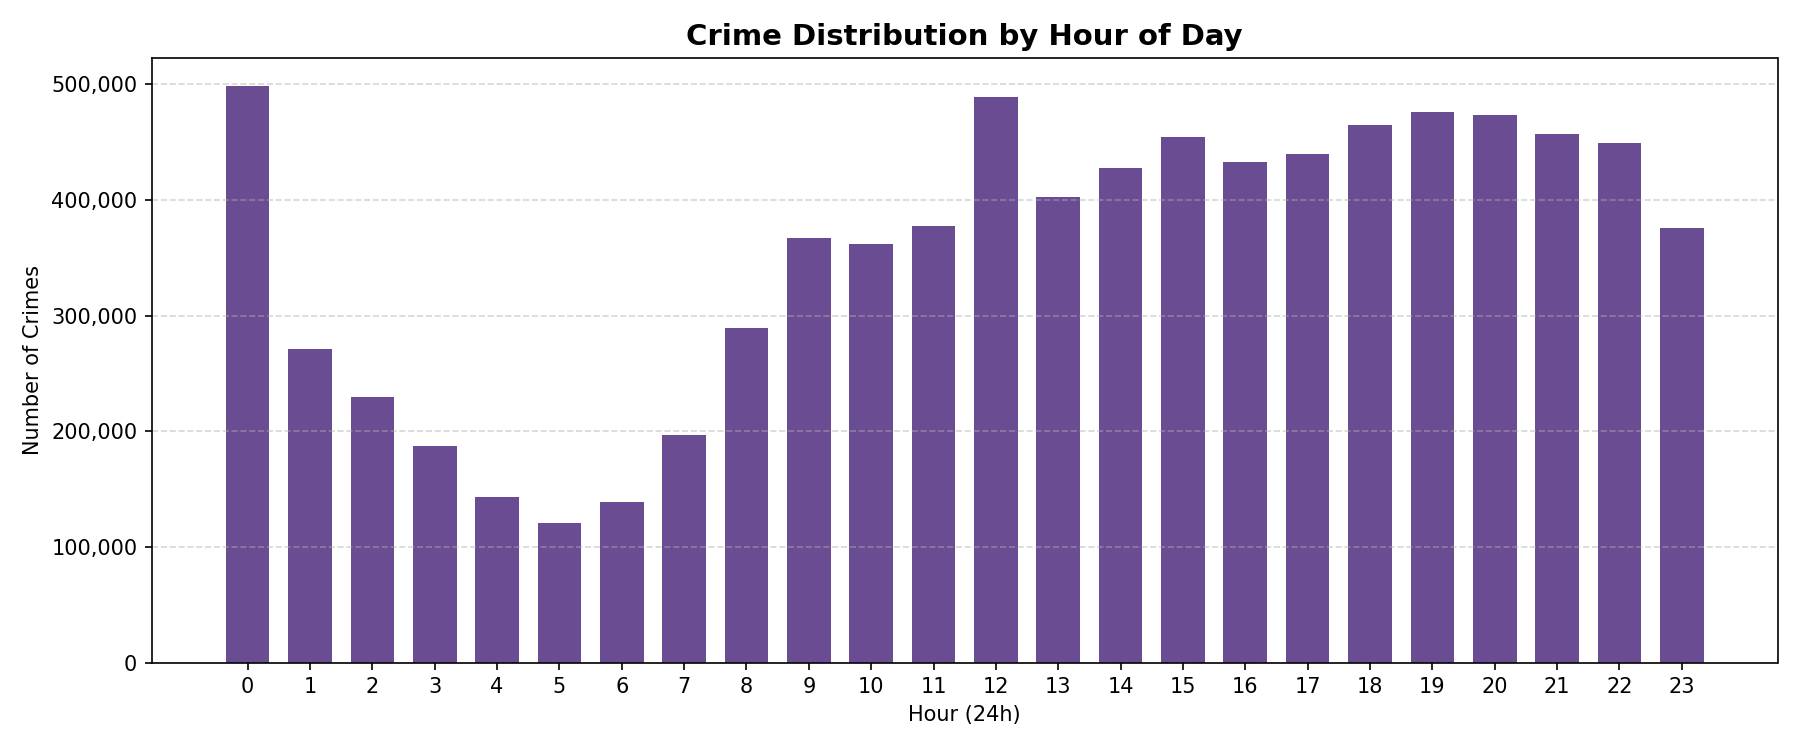
\includegraphics[width=\columnwidth]{crimes_by_hour.png}
\caption{Crime distribution by hour of day (24-hour clock). The midnight peak
(498,321 incidents) and the 05:00 trough (120,377) define the primary temporal
rhythm of criminal activity in Chicago.}
\label{fig:hour}
\end{figure}

\begin{figure}[H]
\centering
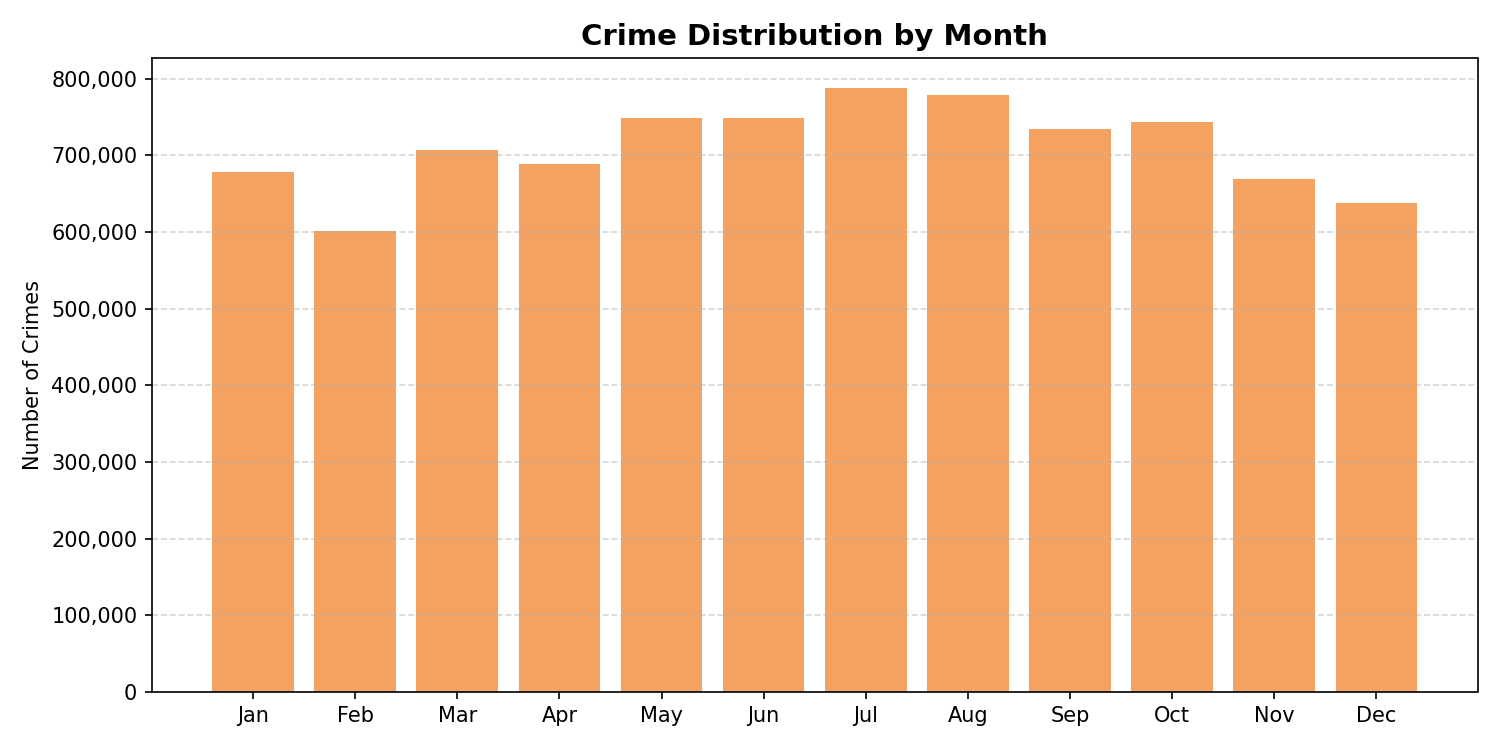
\includegraphics[width=\columnwidth]{crimes_by_month.png}
\caption{Crime distribution by month. Summer months (July--August) record
approximately 31\% more incidents than the winter minimum (February).}
\label{fig:month}
\end{figure}

\begin{figure}[H]
\centering
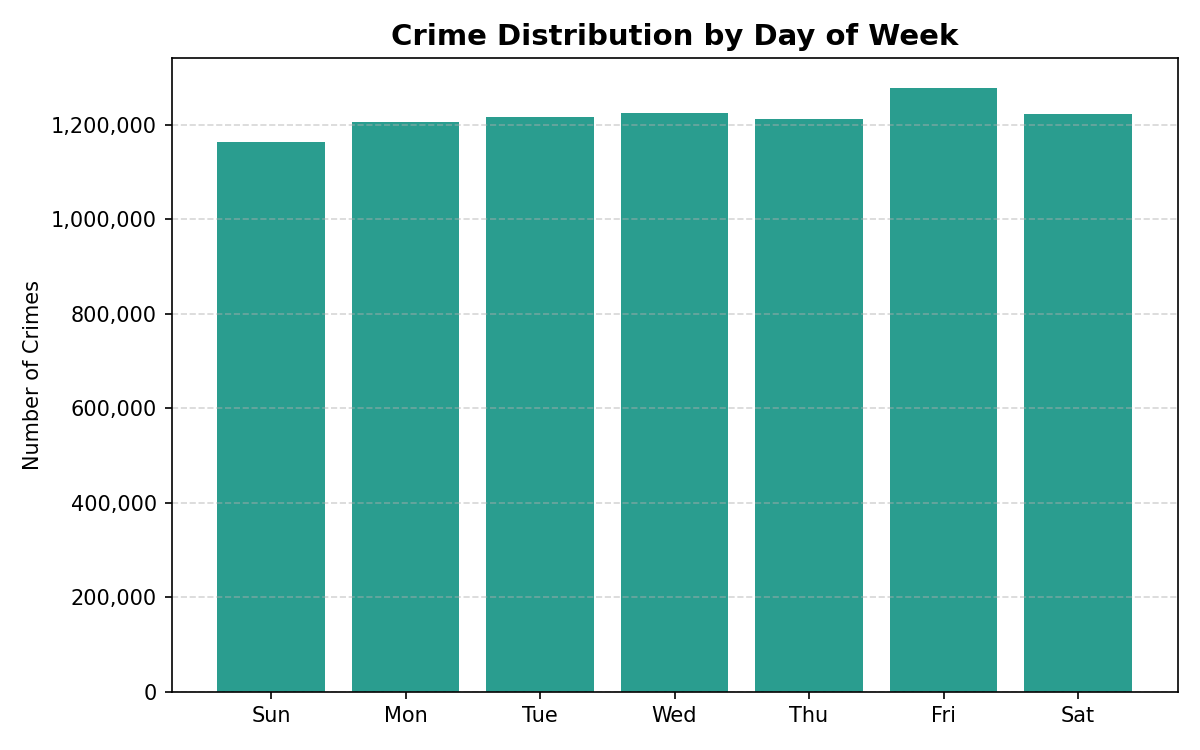
\includegraphics[width=\columnwidth]{crimes_by_dow.png}
\caption{Crime distribution by day of week. Friday is the peak day (1,278,678);
Sunday the lowest (1,163,862). Variation across days is modest compared to
hour-of-day differences.}
\label{fig:dow}
\end{figure}

\subsection{Geographic Distribution}

District 8 (Austin neighbourhood) records the highest crime volume (571,465),
followed by District 11 (Harrison, 539,808) and District 6 (Gresham, 497,939).
These three districts account for 18.9\% of all incidents while covering a fraction
of the city's geographic area.

By location type, streets (2,228,091) and residences (1,395,413) account for 42.6\%
of all incidents. Sidewalks (766,756) and apartments (1,022,007) are also significant
venues.

\subsection{Domestic Crime}

Of 8,525,498 total incidents, 1,473,550 (17.3\%) are classified as domestic crimes.
The remaining 7,051,948 (82.7\%) are non-domestic. This proportion is consistent
with national domestic violence reporting statistics and suggests that domestic
incidents constitute a significant but minority share of overall law enforcement
demand.

\begin{figure}[H]
\centering
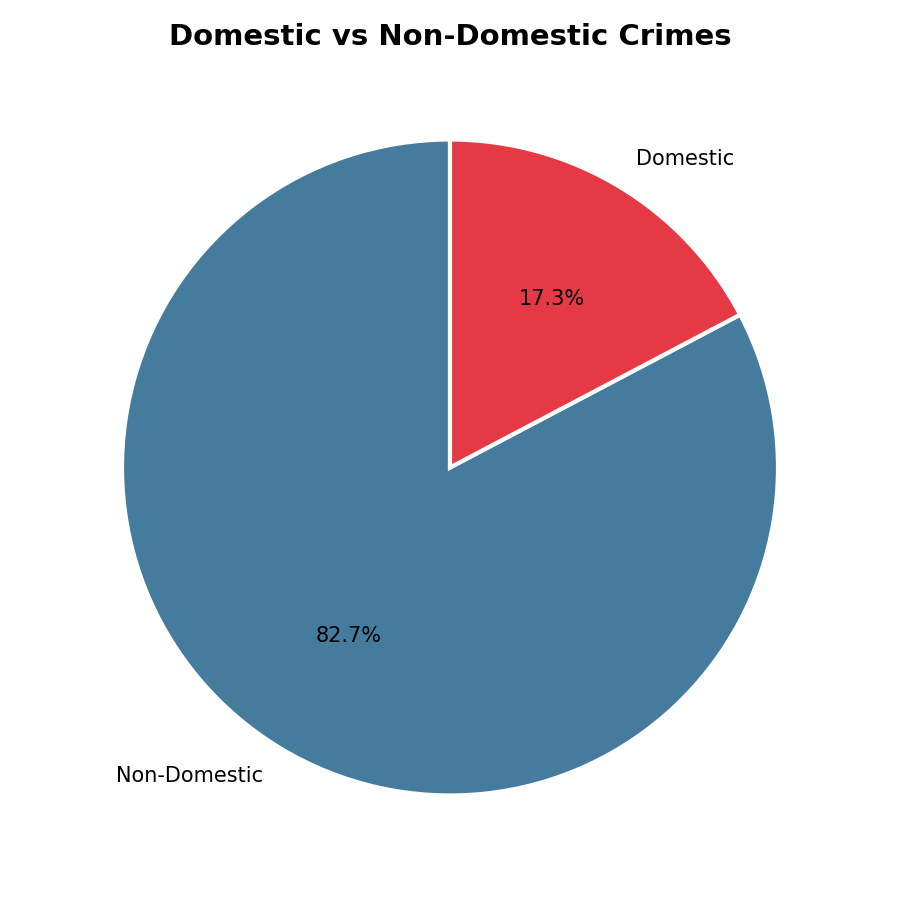
\includegraphics[width=0.75\columnwidth]{domestic_pie.png}
\caption{Domestic vs.\ non-domestic crime split across all 8,525,498 incidents.
Domestic incidents account for 17.3\% of total reported crimes.}
\label{fig:domestic}
\end{figure}

\subsection{Predictive Model}

The linear regression model trained on 2001--2019 data estimated a trend slope of
\textbf{$-$15,172 crimes per year}, meaning Chicago averaged approximately 15,000
fewer crimes annually during the pre-pandemic period. On the 2020--2025 test set,
the model produced an $R^2$ of $-10.62$ and MAE of 57,580 crimes/year, indicating
that the linear model fails to capture the COVID disruption and subsequent rebound.

This negative $R^2$ is itself an informative finding: the period 2020--2025
constitutes a structural break in the crime trend, driven by pandemic-era social
disruption rather than the gradual deterrence effects modelled by the training data.
The forecast for 2026--2030 (assuming a return to the pre-pandemic trend) projects
annual crime volumes declining from approximately 128,555 in 2026 to 67,866 in
2030, though these figures should be interpreted with significant caution given
the model's poor test performance.

More sophisticated time-series models (ARIMA, LSTM) that can accommodate structural
breaks would substantially improve forecast accuracy and are recommended for
operational use.

\begin{figure}[H]
\centering
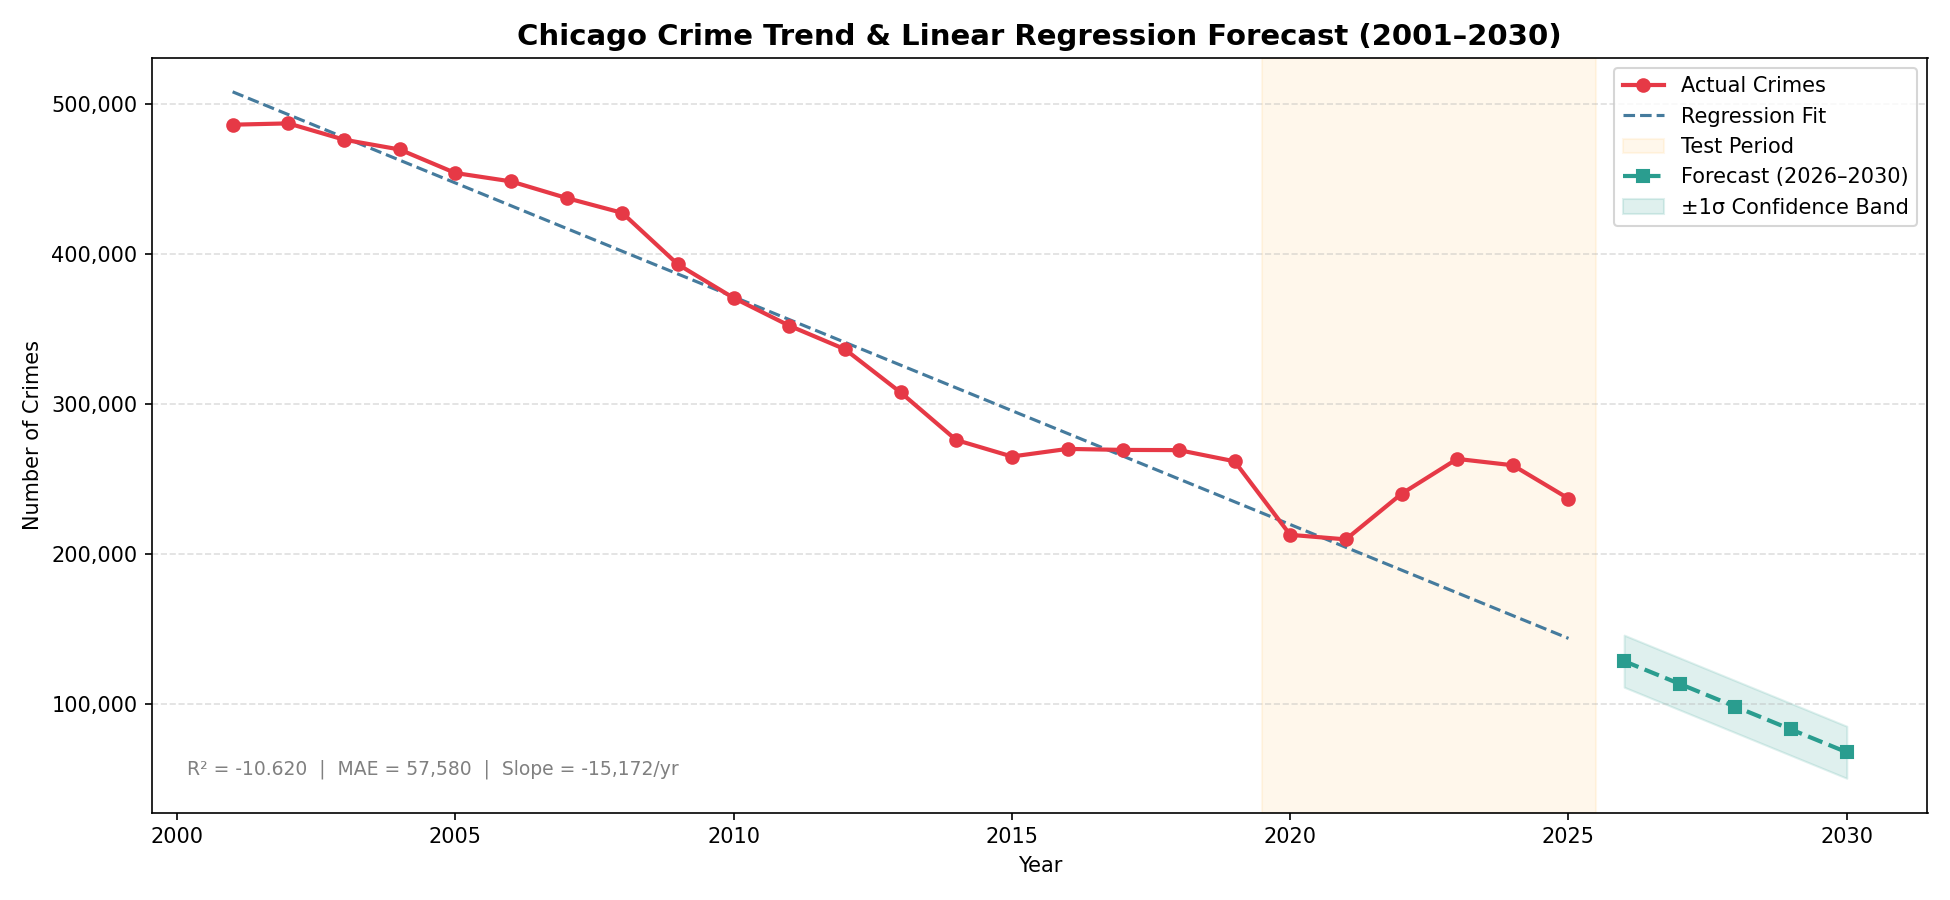
\includegraphics[width=\columnwidth]{crime_forecast.png}
\caption{Linear regression crime forecast (2026--2030) trained on 2001--2019 data.
The shaded orange region indicates the test period (2020--2025). The green dashed
line shows the forecast with $\pm1\sigma$ confidence band. The structural break
caused by COVID-19 is clearly visible.}
\label{fig:forecast}
\end{figure}

\subsection{Crime Type Classification (Advanced AI Prediction)}

To address the limitations of simple linear forecasting, an advanced multiclass
classifier was implemented using Spark MLlib. The model aims to predict the
\textit{Primary Type} of crime (from the top 10 categories) given contextual
features: hour of day, day of week, month, district, ward, community area,
location description, and domestic status.

A Random Forest Classifier with 100 trees and a maximum depth of 10 was trained
on a 20\% stratified sample (approximately 1.7 million records). The model
achieved an overall \textbf{Accuracy of 39.55\%} and an \textbf{F1-score of 0.3155}.
Given that a random baseline (always guessing "Theft") would achieve only
approximately 21\% accuracy, the Spark-based classifier represents a nearly
two-fold improvement in predictive power using only historical context.

Analysis of feature importance (Fig.~\ref{fig:importance}) reveals that
\textit{Domestic Status} (43.0\%) and \textit{Location Description} (39.0\%) are the
dominant predictors of crime type, together accounting for 82\% of the model's
decision weight. Temporal features (Hour: 5.2\%) and geographic markers (Ward: 4.8\%,
Community Area: 4.4\%) provided secondary but significant predictive signals.

\begin{figure}[H]
\centering

\includegraphics[width=\columnwidth]{feature_importance.png}
\caption{Feature importance scores for the Random Forest crime type classifier.
Domestic status and physical location type are the strongest indicators of the
specific crime type likely to occur.}
\label{fig:importance}
\end{figure}

% -------------------------------------------------------
\section{Limitations and Future Work}

Several limitations constrain the current implementation. First, the pipeline
operates in pseudo-distributed mode on a single physical node, which limits
scalability beyond the current dataset size. A genuine multi-node cluster would
be required for real-time streaming ingestion. Second, the linear regression
forecasting model is insufficient for capturing non-linear trend breaks as
demonstrated by the COVID period. Third, geographic analysis in this work is
limited to district-level aggregation; block-level or GPS-coordinate-based
kernel density estimation would yield more operationally useful hotspot maps.

Future work should incorporate: (1) an ARIMA or Prophet model for time-series
forecasting with structural break handling; (2) spatial analysis using GIS
integration with block-level coordinate data already present in the dataset;
(3) a streaming pipeline using Apache Kafka and Spark Structured Streaming for
near-real-time incident analysis; and (4) feature engineering to support
multi-class crime prediction using gradient boosted classifiers.

% -------------------------------------------------------
\section{Conclusion}

This paper presented a complete big data pipeline for urban crime analysis using
Apache Hadoop and PySpark on the Chicago Crimes dataset (8,525,498 records,
2.3~GB). Three Hadoop Streaming MapReduce jobs and six PySpark analyses produced
quantitative findings across temporal, geographic, and categorical dimensions. Key
results include a 56.8\% decline in annual crime from 2001 to 2021, a midnight
crime peak, extreme variation in arrest rates across crime types (5.7\%--99.55\%),
and the identification of three high-crime districts that account for nearly 19\%
of all incidents.

The integration of an advanced Random Forest classifier demonstrated that contextual
features such as domestic status and location type can predict specific crime types
with 39.6\% accuracy, nearly double the performance of a naive baseline. While the
linear regression forecast identified a pre-pandemic decline of 15,172 crimes per year,
the structural break of 2020 highlights the need for more complex ensemble models.
The pipeline demonstrates that open-source distributed computing infrastructure
on commodity hardware is viable for processing multi-million record public safety
datasets and generating actionable analytical insights.

% -------------------------------------------------------
\begin{thebibliography}{00}

\bibitem{chicagoportal}
City of Chicago, ``Crimes -- 2001 to Present,'' Chicago Data Portal, 2024.
[Online]. Available: \url{https://data.cityofchicago.org/Public-Safety/Crimes-2001-to-Present/ijzp-q8t2}

\bibitem{wang2013}
S. Wang, L. Zhong, and E. Wan, ``MapReduce-based large-scale urban event data
processing for crime analysis,'' \textit{IEEE Transactions on Knowledge and Data
Engineering}, vol. 25, no. 5, pp. 1100--1113, 2013.

\bibitem{chainey2008}
S. Chainey, L. Tompson, and S. Uhlig, ``The utility of hotspot mapping for
predicting spatial patterns of crime,'' \textit{Security Journal}, vol. 21,
no. 1--2, pp. 4--28, 2008.

\bibitem{perry2013}
W. L. Perry, B. McInnis, C. C. Price, S. C. Smith, and J. S. Hollywood,
\textit{Predictive Policing: The Role of Crime Forecasting in Law Enforcement
Operations}. Santa Monica, CA: RAND Corporation, 2013.

\bibitem{ahishakiye2021}
E. Ahishakiye, M. B. Van Kamp, J. Niyonzima, and E. Nzeyimana, ``A survey on
crime prediction techniques using machine learning,'' \textit{Journal of Intelligent
\& Fuzzy Systems}, vol. 41, no. 4, pp. 4921--4935, 2021.

\bibitem{malathi2011}
A. Malathi and S. S. Baboo, ``An enhanced algorithm to predict a future crime
using data mining,'' \textit{International Journal of Computer Applications},
vol. 21, no. 1, pp. 1--6, 2011.

\end{thebibliography}

\end{document}